\chapter{Fundamentação Teórica}
\label{cap:fundamentacao}
Neste capítulo serão apresentados os conceitos teóricos que são base para este trabalho. Primeiramente será introduzido o funcionamento básico das redes neurais e das redes neurais profundas. Em seguida, será apresentado o conceito de aprendizado de máquina, onde serão definidas as técnicas de aprendizado supervisionado, não supervisionado e por reforço. Depois, será definido em mais detalhes a motivação e os tipos de aprendizado por reforço, assim como a Estimativa de Vantagem Generalizada e o algoritmo \textit{Proximal Policy Optimization} que são utilizados como ferramenta neste trabalho. Por fim, serão apresentadas os principais problemas relacionados a ambientes com recompensa esparsa no contexto de aprendizado por reforço e será introduzida a técnica de exploração por curiosidade e motivação intrínseca.

%% - - - - - - - - - - - - - - - - - - - - - - - - - - - - - - - - - - -

\section{Redes Neurais}
\label{sec:redesneurais}

Redes Neurais Artificiais (RNAs) são técnicas computacionais para modelagem matemática inspiradas pelo sistema nervoso central de organismos inteligentes. RNAs são tipicamente utilizadas como aproximadoras de funções universais e possuem estruturas que fazem um paralelo entre mecanismos biológicos como neurônios, sinapses e diferentes organizações estruturais (topologias) \cite{Russel}. 

% \subsection{Neurônio}

\begin{figure}[ht]
 \centering
  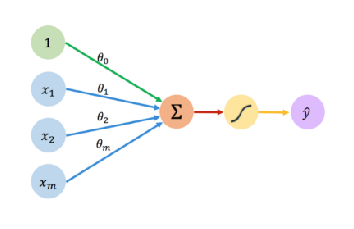
\includegraphics[width=0.5\textwidth]{./fig/Neuron}
  \caption{Diagrama do funcionamento de um neurônio.}
 \label{fig:neuron}
\end{figure}

A unidade mais básica de processamento de uma rede neural é o neurônio, que recebe um ou mais valores $x_i$ como entrada, multiplica-os pelo peso sináptico correspondente $\theta_i$ e adiciona sua soma a um valor $b$ conhecido como \textit{bias} \cite{Goodfellow2016}. O valor final é alimentado a uma função de ativação que induz a não-linearidade da função aproximada pelo sistema. Este processo é demonstrado na Figura \ref{fig:neuron}.

De uma forma mais didática, o parâmetro $\theta_i$ define quanto de um sinal $x_i$ deverá ser considerado no processamento do neurônio e $b$ permite que o neurônio ajuste o sinal de saída de uma forma independente dos sinais de entrada. A função de ativação permite o neurônio representar funções mais complexas que funções lineares \cite{Luckeciano}. A Equação \ref{eqn:neuron} descreve o processamento de um neurônio.

\begin{equation}
\label{eqn:neuron}
\hat{y} = \sigma(w^Tx+b)
\end{equation}

Dentre as funções de ativação mais utilizadas na prática estão a \textit{Rectified Linear Unit} (ReLU), a tangente hiperbólica (TanH) e a função sigmóide, utilizada na Equação \ref{eqn:neuron}. Cada função de ativação possui um comportamento específico, que pode ser observado na Figura \ref{fig:activationfunctions}.

\begin{figure}[ht]
 \centering
  \subfigure[ReLU.]
   {
    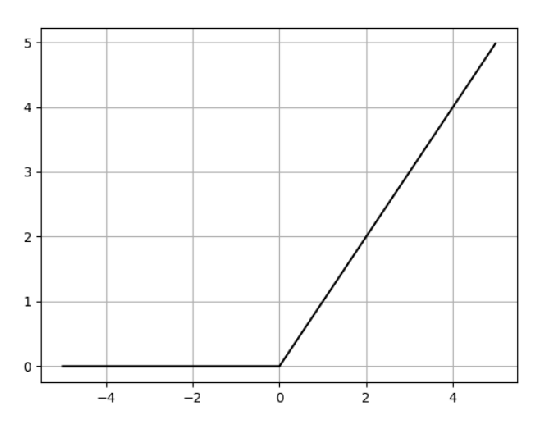
\includegraphics[width=0.277\textwidth]{./fig/ReLU}
    \label{subfig:relu}
   }
   \subfigure[TanH.]
   {
    \includegraphics[width=0.3057\textwidth]{./fig/TanH}
    \label{subfig:tanh}
   }
  \subfigure[Sigmóide.]
   {
    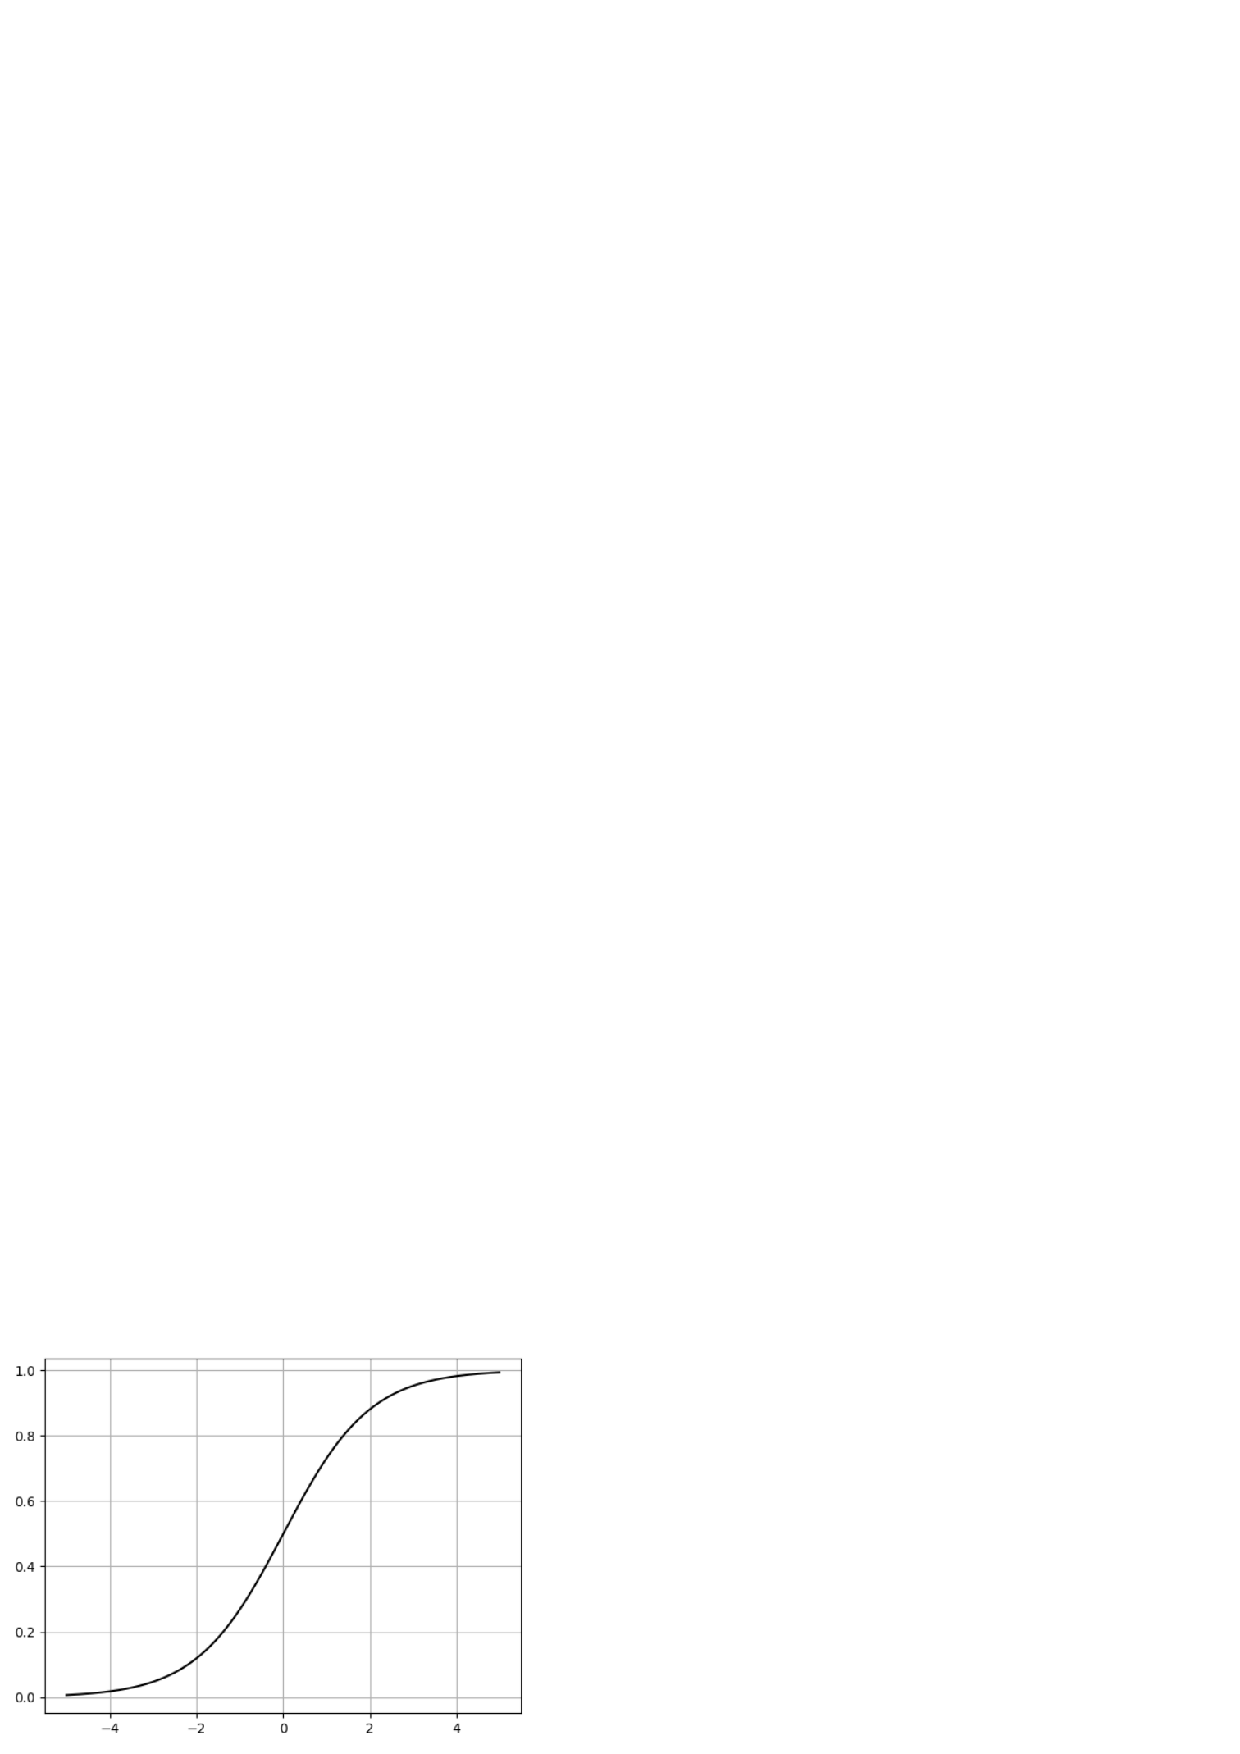
\includegraphics[width=0.3\textwidth]{./fig/Sigmoid}
    \label{subfig:sigmoid}
   }
   \captionsetup{width=1\textwidth}
   \caption{{\subref{subfig:relu}}, {\subref{subfig:tanh}} e {\subref{subfig:sigmoid}} representam o comportamento das funções de ativação ReLU, TanH e Sigmóide, respectivamente \cite{Luckeciano}.}
  \label{fig:activationfunctions}
\end{figure}

% \subsection{Topologia}
Uma rede neural combina diversos neurônios em diversas camadas, formando um grafo direcionado (tipicamente acíclico) por onde os dados fluem. Os neurônios de uma camada processam os dados de entrada e passam os resultados como entrada dos neurônios da próxima camada, até encontrar a camada de saída \cite{MichaelNielsen}. Uma rede neural que possui muitas camadas é denominada uma Rede Neural Profunda. A Figura \ref{fig:neuralnetworks} ilustra o fluxo de processamento de redes neurais.

\begin{figure}[ht]
 \centering
  \subfigure[Rede neural.]
   {
    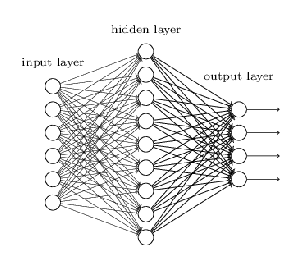
\includegraphics[width=0.35\textwidth]{./fig/NeuralNetwork}
    \label{subfig:nn}
   } \qquad
  \subfigure[Rede neural profunda.]
   {
    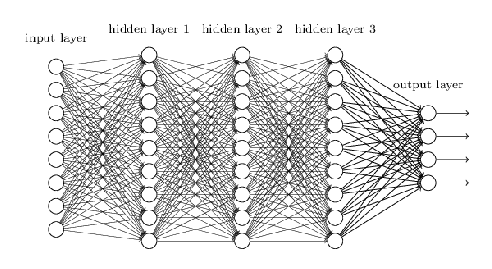
\includegraphics[width=0.55\textwidth]{./fig/DNN}
    \label{subfig:deepnn}
   }
   \captionsetup{width=1\textwidth}
   \caption{{\subref{subfig:nn}} e {\subref{subfig:deepnn}} representam uma rede neural convencional e uma rede neural profunda, respectivamente \cite{MichaelNielsen}.}
  \label{fig:neuralnetworks}
\end{figure}

Existem diversas topologias para redes neurais que não seguem necessariamente a configuração apresentada. Redes Neurais Convolucionais, por exemplo, utilizam filtros convolucionais para extrair características em conjuntos de entradas onde a posição dos elementos é importante (e.g. imagens) \cite{LeCun1989} e Redes Neurais Recorrentes definem grafos cíclicos para modelagem de dados em domínios temporais \cite{Rumelhart1986}. As camadas de uma rede neural podem ter todos os seus neurônios conectados a todos os neurônios da camada anterior - as camadas densas - ou podem ter conexões compartilhadas, como é o caso dos filtros convolucionais \cite{LeCun1989}.

\begin{figure}[ht]
 \centering
  \subfigure[Topologia de uma Neural Convolucional.]
   {
    \includegraphics[width=0.55\textwidth]{./fig/CNN}
    \label{subfig:convnn}
   } \qquad
  \subfigure[Topologia de uma Rede Neural Recorrente.]
   {
    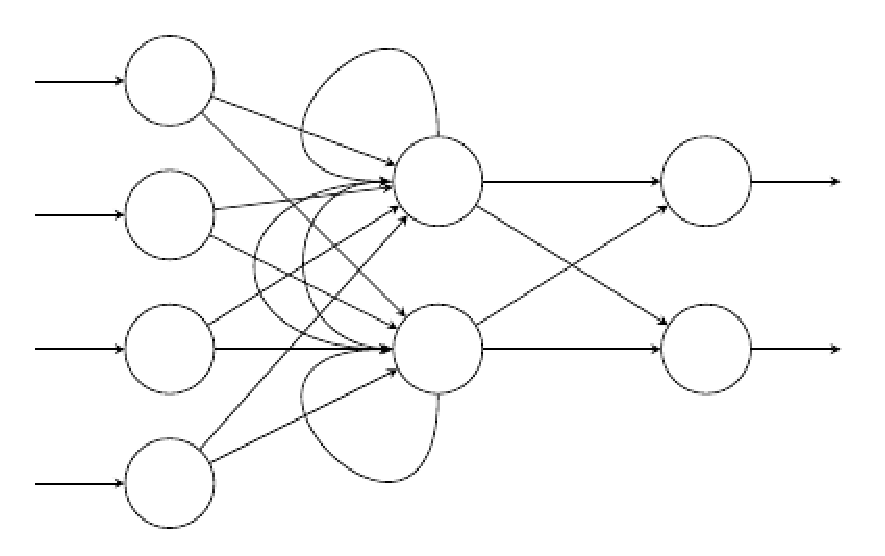
\includegraphics[width=0.35\textwidth]{./fig/RNN}
    \label{subfig:rnn}
   }
   \captionsetup{width=1\textwidth}
   \caption{{\subref{subfig:convnn}} e {\subref{subfig:rnn}} representam diferentes topologias que redes neurais podem assumir.}
  \label{fig:topologies}
\end{figure}

% \subsection{Otimização}

A otimização, ou treinamento, de redes neurais é uma tarefa natural do aprendizado supervisionado, que será introduzido em seguida. Os algoritmos mais utilizados para isso são baseados na propagação do gradiente de uma função de custo através da rede a fim de atualizar seus parâmetros e minimizar esta função, um processo conhecido como \textit{backpropagation} \cite{Goodfellow2016}.

%% - - - - - - - - - - - - - - - - - - - - - - - - - - - - - - - - - - -

\section{Aprendizado de Máquina}
\label{sec:aprendizadomaquina}

Aprendizado de máquina é um subcampo da Inteligência Artificial que estuda a capacidade de algoritmos aprenderem a executar tarefas baseadas em dados sem que sejam explicitamente programados para tal \cite{Simon2013TooBT}. Na prática, seu objetivo é modelar teórica e matematicamente o processo de melhoria interativa das aplicações, baseando-se em padrões intrínsecos dos dados disponíveis. Existem três principais técnicas para alcançar este objetivo: aprendizado supervisionado, aprendizado não supervisionado e aprendizado por reforço. 

No aprendizado supervisionado pares de exemplos no formato $(X, Y)$, onde $X$ são entradas e $Y$ são saídas, são dados ao algoritmo para que este consiga aproximar uma função $f$ que mapeie uma entrada $x \in X$ à saída correspondente $y \in Y$ \cite{Russel}. Algoritmos de aprendizado supervisionado podem ainda ser classificados entre algoritmos de classificação e algoritmos de regressão, onde o primeiro mapeia uma entrada $x$ a uma das classes em $Y$ e o segundo mapeia uma entrada $x$ em um valor contínuo no domínio de $Y$.

No aprendizado não supervisionado, por sua vez, o aprendizado é feito sobre dados não anotados, ou seja, sem o conjunto $Y$. O objetivo dessa classe de algoritmos é extrair padrões e regras, agrupar ou resumir os dados \cite{Russel}.

Já no aprendizado por reforço o aprendizado ocorre através da interação com um ambiente. Uma solução para um problema de aprendizado por reforço - o agente - deve interagir com o ambiente executando ações que geram sinais de recompensa. Dessa forma, o agente, em busca de maximizar o valor total da soma de suas recompensas futuras, deve aprender comportamentos (políticas) que ao mesmo tempo resolvem o problema inicialmente proposto \cite{Russel}. A Figura \ref{fig:reinforcementfig} representa o processo descrito. Esta abordagem é descrita em mais detalhes na Seção \ref{sec:reinforcementlearning}.
\begin{figure}[ht]
 \centering
  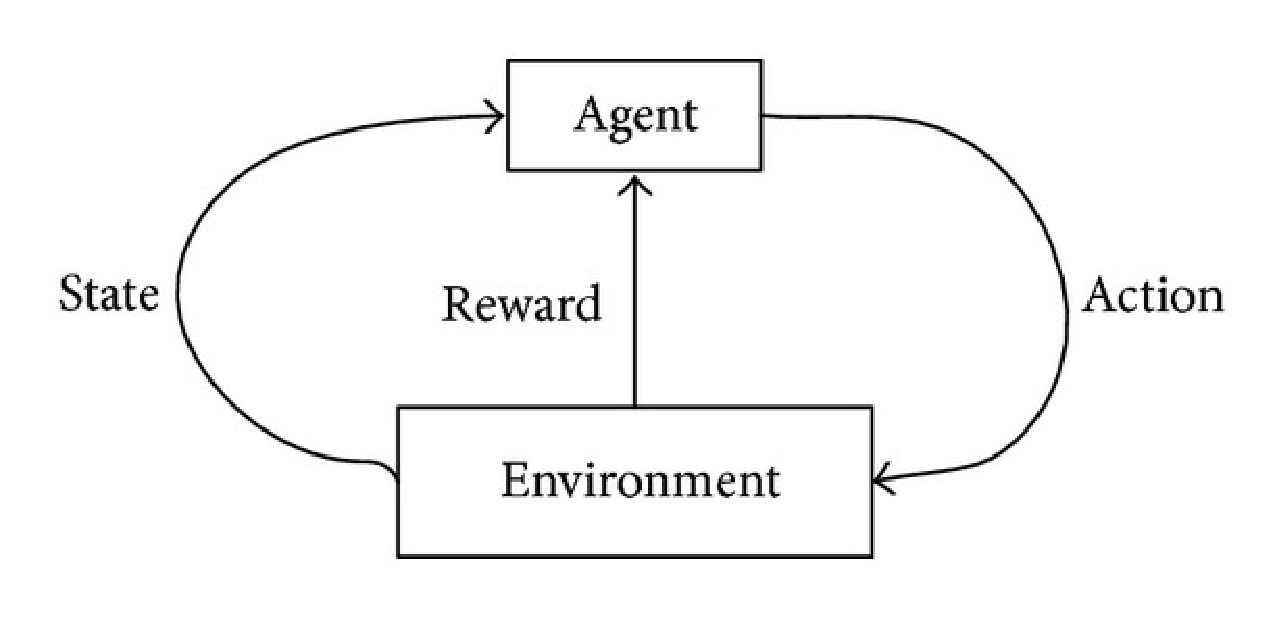
\includegraphics[width=0.70\textwidth]{./fig/Framework-of-reinforcement-learning-Agent-selects-an-action-the-environment-responds-to}
  \captionsetup{width=1\textwidth}
  \caption[Diagrama do processo de aprendizado por reforço \cite{ZhouXiaoke}.]{Diagrama do processo de aprendizado por reforço \cite{ZhouXiaoke}. Um agente (\textit{Agent}), em um dado estado (\textit{State}), seleciona ações (\textit{Action}) que são aplicadas no ambiente (\textit{Environment}) que, por sua vez, retorna um novo estado e um sinal de recompensa (\textit{Reward}) para o agente.}
 \label{fig:reinforcementfig}
\end{figure}

%% - - - - - - - - - - - - - - - - - - - - - - - - - - - - - - - - - - -

\section{Aprendizado por Reforço}
\label{sec:reinforcementlearning}

No aprendizado por reforço, um agente aprende através de sua interação com o ambiente em sequências de iterações, chamadas de episódios. Essa interação é tipicamente modelada como um Processo de Decisão de Markov (MDP), definido por um conjunto de estados $S$, um espaço de ações $A$, uma função de recompensa $r: S \times A \rightarrow [-\infty, \infty)$, um fator de desconto $\gamma \in [0, 1)$ e uma função de transição $P: S \times A \rightarrow \Delta(S)$. Nessa configuração, $\Delta(S)$ é o espaço de distribuições de probabilidade $P(s'|s, a)$ de transição para um estado $s'$ a partir de um estado $s$ e executando a ação $a$. O fator de desconto $\gamma$ é utilizado para balancear quanto um agente deve priorizar recompensas imediatas ou recompensas futuras. A Figura \ref{fig:mdp} ilustra o sistema descrito.

\begin{figure}[ht]
 \centering
  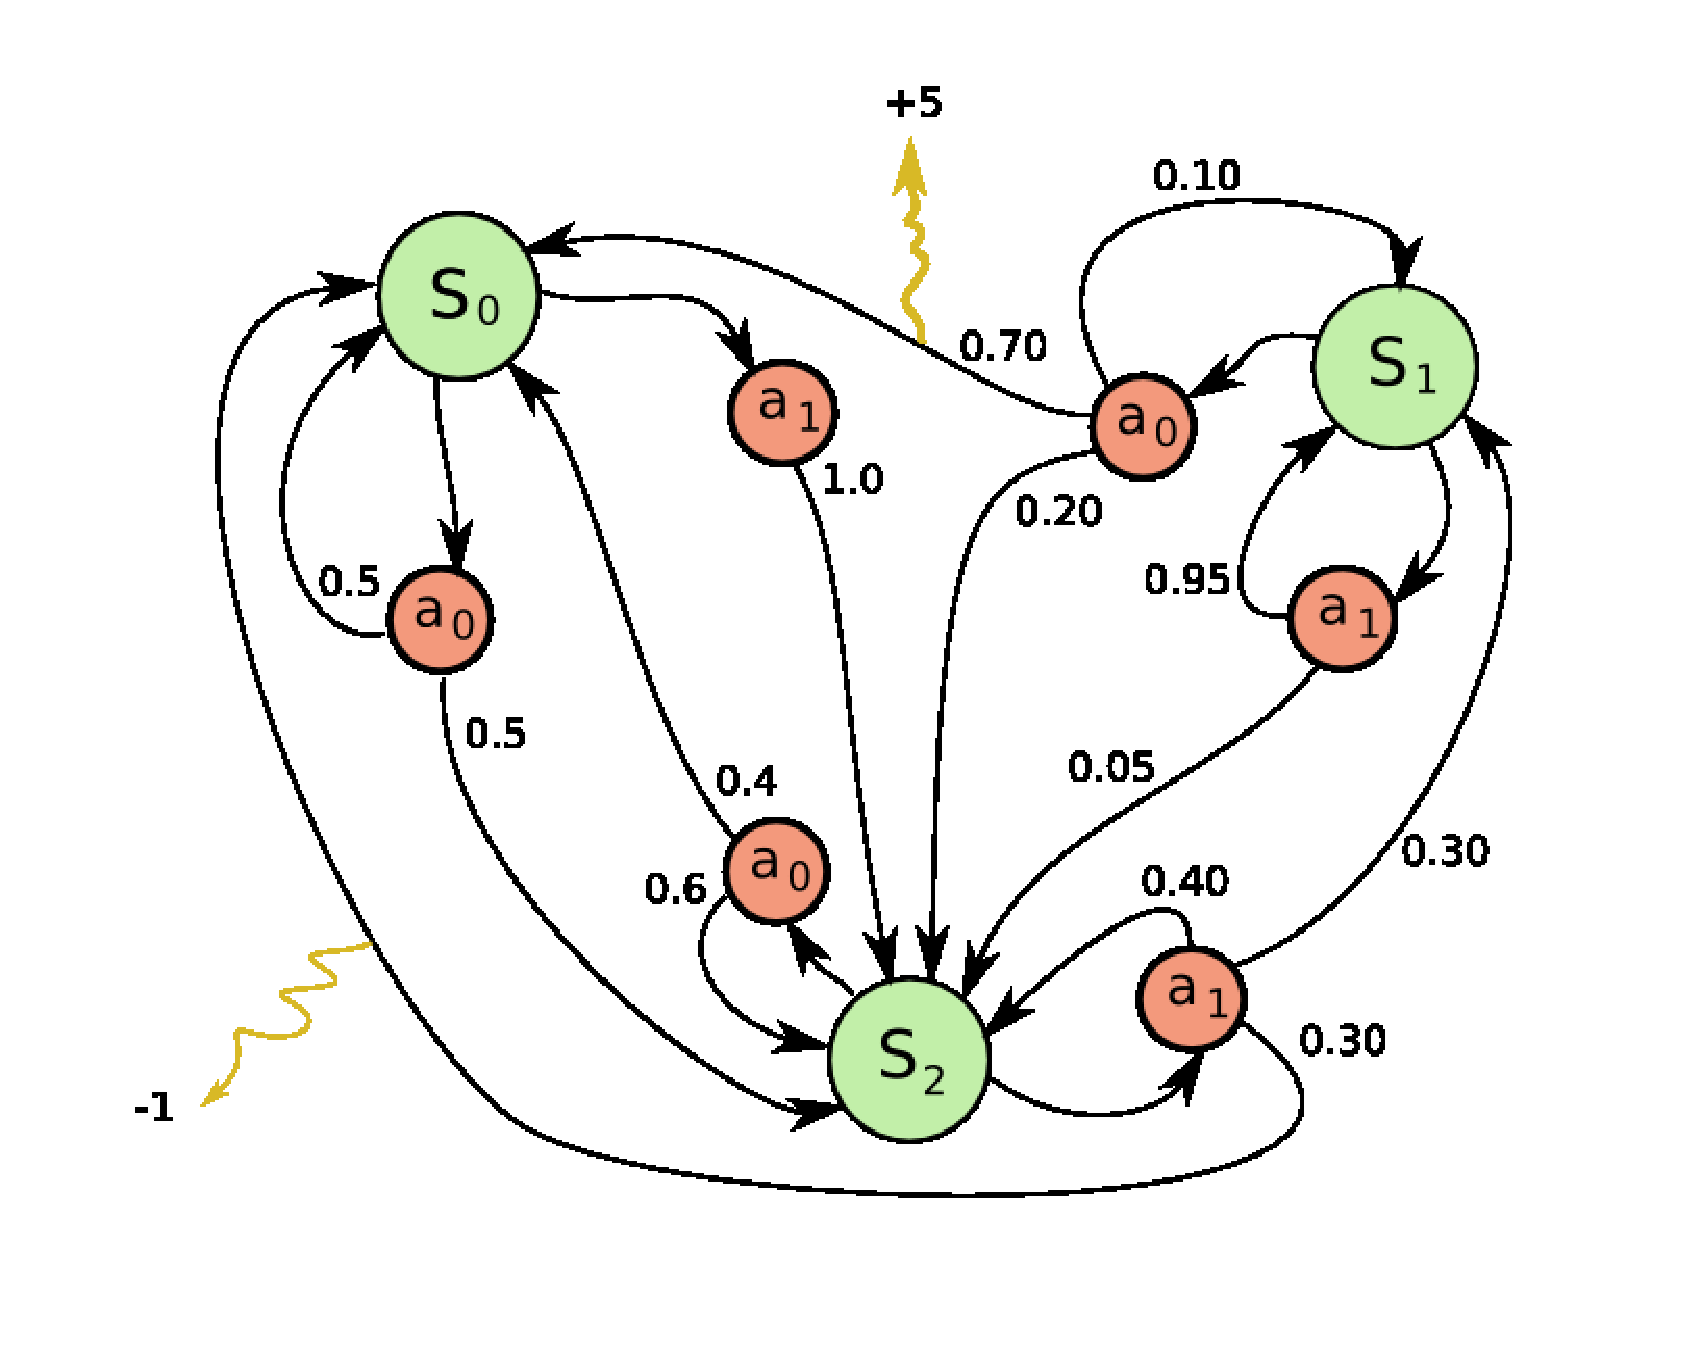
\includegraphics[width=0.6\textwidth]{./fig/mdp}
  \captionsetup{width=1\textwidth}
  \caption[Um Processo de Decisão de Markov \cite{mohammad}.]{Um Processo de Decisão de Markov \cite{mohammad}. Os estados $s_i \in S$ e as ações $a_i \in A$ são representadas pelos vértices verdes e vermelhos, respectivamente. Os valores das arestas são as probabilidades de transição $P$ e os valores indicados pelas setas amarelas são as recompensas obtidas em cada transição.}
 \label{fig:mdp}
\end{figure}

Sequências de transições em um MDP formam uma cadeia de Markov \cite{drlhandson}. O valor total de recompensas, ou retorno, que um agente pode receber em uma cadeia a partir de um tempo $t$ é definido pela Equação \ref{eqn:rewards}.

\begin{equation}
\label{eqn:rewards}
R_t = r_{t+1} + \gamma r_{t+2} + ... = \sum^\infty_{k=0}{\gamma^k r_{t+k+1}}
\end{equation}

Na prática, diferentes cadeias de transições podem resultar no mesmo valor de $R_t$. Como o objetivo de um agente de aprendizado por reforço é maximizar o retorno para uma cadeia qualquer, definimos, para esse fim, a função de valor $V$ para um estado $s$, como mostra a Equação \ref{eqn:value}. O valor de um estado, portanto, pode ser definido como o valor esperado da recompensa que pode ser acumulada a partir do estado atual, independentemente da sequência exata de transições que ocorreram.

\begin{equation}
\label{eqn:value}
V(s) = \mathop{{}\mathbb{E}} [R | S_t=s]
\end{equation}

O agente seleciona suas ações baseando-se em sua política, que pode ser determinística, como na Equação \ref{eqn:pidet}, ou estocástica, como na Equação \ref{eqn:piest}. Tipicamente, políticas determinísticas são utilizadas em ambientes determinísticos, como o jogo de xadrez, enquanto que políticas estocásticas são amplamente utilizadas em ambientes estocásticos, como em um jogo de poker, modelados como Processos de Decisão de Markov Parcialmente Observáveis (PDMPO) \cite{drlhandson}. Em MDPs, a observação do estado atual é suficiente para que um agente obtenha uma política ótima, ou seja, é suficiente para que seja possível alcançar o objetivo de maximizar sua recompensa acumulada. PDMPOs, por outro lado, possuem variáveis escondidas que tornam essa tarefa significativamente difícil e, portanto, são abordados com estratégias mais sofisticadas.

\begin{equation}
\label{eqn:pidet}
\pi(s) = a
\end{equation}

\begin{equation}
\label{eqn:piest}
\pi(a|s) = P(A_t=a | S_t=s)
\end{equation}

Um agente pode otimizar seu comportamento melhorando sua estimativa do valor de um par estado-ação (métodos baseados em valor) ou modificando sua política (métodos baseados em política). Além disso, um agente pode armazenar e otimizar um modelo do ambiente internamente (baseado em modelo) para consultá-lo na tomada de decisões ou trabalhar sem conhecer o funcionamento interno do ambiente (livre de modelo). Outro tipo de classificação especifica se o agente utiliza informações da própria política exploratória para otimização em direção à política ótima (\textit{on-policy}) ou não (\textit{off-policy}) \cite{suttonbarto}.

Agentes modernos de aprendizado por reforço tipicamente utilizam redes neurais como forma de parametrizar seus componentes. Isso permite que o agente trabalhe com espaços de observação e ação contínuos e de alta dimensionalidade. Esses agentes são comumente denominados agentes de aprendizado por reforço profundo. Uma política parametrizada por parâmetros $\theta$ é denotada por $\pi_\theta$.

Enxergando a otimização de agentes como um problema de maximização de recompensa acumulada, técnicas de exploração dão ao agente a possibilidade de sair de máximos locais ao explorar novos estados do ambiente. Uma das políticas exploratórias mais utilizadas é o $\epsilon$-\textit{greedy} \cite{egreedy}. Nessa técnica, o agente seleciona a ação de maior valor estimado com probabilidade $1-\epsilon$ ou uma ação aleatória com probabilidade $\epsilon$, como é feito em \cite{deepq}. Ao decorrer do processo de treinamento, o parâmetro $\epsilon$ é reduzido até que somente a política do agente seja utilizada na seleção de ações. 

Em métodos baseados em política, a exploração pode ser feita através da seleção da ação por amostragem em uma distribuição de probabilidades gerada pela política. Nesse método, a ação executada em um estado pode variar, mas de forma controlada. Outra forma de encorajar a exploração em métodos baseados em política é a adição de um termo de regularização baseado na entropia ($H(\pi(s_t; \theta))$) da distribuição gerada pelo agente na função de custo do problema de otimização da política \cite{a3c, williamspeng}. Isso faz com que o agente prefira distribuições mais uniformes a distribuições que encorajam demais as mesmas ações, evitando a convergência (ou seja, a estabilização em resultados relativamente satisfatórios) para políticas sub-ótimas e mantendo um nível controlado de exploração \cite{a3c, williamspeng}.

\section{Estimativa de Vantagem Generalizada}
\label{sec:gae}

Métodos baseados em política possuem a vantagem de aprender políticas estocásticas, ao contrário de métodos baseados em valor. Além disso, esses métodos conseguem trabalhar em espaços de ação de alta dimensionalidade, ou contínuos, por poderem ser representados por qualquer aproximador parametrizado que mapeie estados a ações \cite{suttonbarto}. Métodos baseados em política selecionam suas ações sem consultar diretamente uma função de valor, mas comumente as utilizam internamente no processo de otimização. Outra vantagem de utilizar métodos baseados em política é sua garantia de convergência pelo método de Gradiente de Política \cite{policygradients}.

Métodos modernos de Gradiente de Política utilizam como objetivo, assim como os métodos tradicionais de aprendizado por reforço, a maximização da recompensa obtida pelo agente. Para isso, no entanto, é utilizada a Estimativa de Vantagem Generalizada (GAE) \cite{gae}, definida pela Equação \ref{eqn:gae}. Nesse contexto, definimos a vantagem $A$ para um tempo $t$ como a diferença entre a estimativa de valor para o estado atual e o real valor obtido empiricamente. Essa função nos diz se a recompensa obtida foi melhor ($A > 0$) ou pior ($A < 0$) que a recompensa esperada pelo agente. Se for melhor, devemos reforçar as ações executadas no episódio. Se for pior, devemos tornar essas ações menos prováveis.

\begin{equation}
\label{eqn:gae}
A_t^{GAE(\gamma, \lambda)} = (1 - \lambda)(A_t^{(1)} + \lambda A_t^{(2)} + \lambda^2A_t^{(3)} + ...)
\end{equation}

Aqui, $A_t^{GAE(\gamma, \lambda)}$ é um estimador para a função de vantagem generalizada, aplicado no tempo $t$ e configurado pelos hiperparâmetros $\gamma$ e $\lambda$. Os estimadores de vantagem com visão de $n$ passos a partir do tempo $t$ ($A^{(n)}$) são definidos pela Equação \ref{eqn:nstepadv}. O hiperparâmetro $\lambda$ varia de 0 a 1 e controla quanto das estimativas de vantagem para passos futuros devem ser considerados, balanceando o viés e a variação das estimativas \cite{gae}.

\begin{equation}
\label{eqn:nstepadv}
A_t^{(n)}(s, a) = r_t + \gamma V(s_{t+1}) + ... + \gamma^n V(s_{t+n}) - V(s_t)
\end{equation}

O uso de estimadores de vantagem para a otimização nos métodos de Gradiente de Política torna o treinamento mais estável em relação ao uso dos retornos (Equação \ref{eqn:rewards}) para valores de $\lambda$ entre 0 e 1 \cite{gae}.

\section{Proximal Policy Optimization}
\label{sec:ppo}

Um recorrente problema no treinamento de redes neurais é a escolha da taxa de aprendizado. Este parâmetro controla quanto o gradiente influencia na modificação dos parâmetros da rede e é bastante sensível: se for muito grande, a rede pode ser modificada drasticamente e perdemos qualquer conhecimento adquirido até o momento; se for muito pequeno, o treinamento é muito lento.
Esse efeito é ainda maior no aprendizado por reforço, em especial em métodos baseados em política. Leves mudanças nos parâmetros podem levar a grandes mudanças no comportamento do agente, o que torna o treinamento um processo instável.

O algoritmo \textit{Proximal Policy Optimization} (PPO) \cite{ppo} foi introduzido com o propósito de mitigar justamente esse problema, limitando a mudança sofrida pela política entre as atualizações de seus parâmetros. A proporção da atualização da nova política em relação a política anterior é dada pela Equação \ref{eqn:pporatio}.

\begin{equation}
\label{eqn:pporatio}
d_t(\theta) = \frac{\pi_\theta(a_t|s_t)}{\pi_{\theta_{old}}(a_t|s_t)}
\end{equation}

Nesse contexto, se $d_t(\theta)$ > 1, então a ação $a_t$ é mais provável na política atual do que na política antiga. Por outro lado, se $0 < d_t(\theta) < 1$, a ação $a_t$ é menos provável na política atual do que na política antiga. Com base nisso, definimos a função de atualização limitada do PPO na Equação \ref{eqn:ppoloss}, onde \textit{clip} é uma função de corte que restringe $d_t$ ao intervalo $(1-\epsilon, 1+\epsilon)$.

\begin{equation}
\label{eqn:ppoloss}
L^{CLIP}(\theta) = \mathop{{}\mathbb{E}}{}_t [min(d_t(\theta)A_{\pi_\theta}, clip(d_t(\theta), 1-\epsilon, 1+\epsilon) A_{\pi_\theta})]
\end{equation}

Essa função é calculada por N passos de otimização sobre um lote de iterações coletado durante um episódio. Como o objetivo do PPO é garantir pequenas atualizações nos parâmetros $\theta$ a cada episódio, a função de atualização busca o mínimo entre uma atualização para o passo atual com e sem o limite de proporção $\epsilon$. Isso desencoraja a política de desviar muito do que era, uma vez que os gradientes zeram ao ultrapassar a região de corte, como mostra a Figura \ref{fig:ppoclip}. Em outras palavras, se a ação foi boa ($A > 0$) e se tornou mais provável após o último passo de otimização do gradiente, é permitido aumentar sua probabilidade ainda mais até que $d_t$ atinja o limite de corte $1+\epsilon$, ou diminuí-la para reparar erros de passos anteriores. Da mesma forma, se a ação foi ruim ($A < 0$) e se tornou menos provável, é permitido diminuir sua probabilidade até que $d_t$ atinja o limite de corte $1-\epsilon$, ou aumentá-la para reparar erros de passos anteriores.

\begin{figure}[ht]
 \centering
  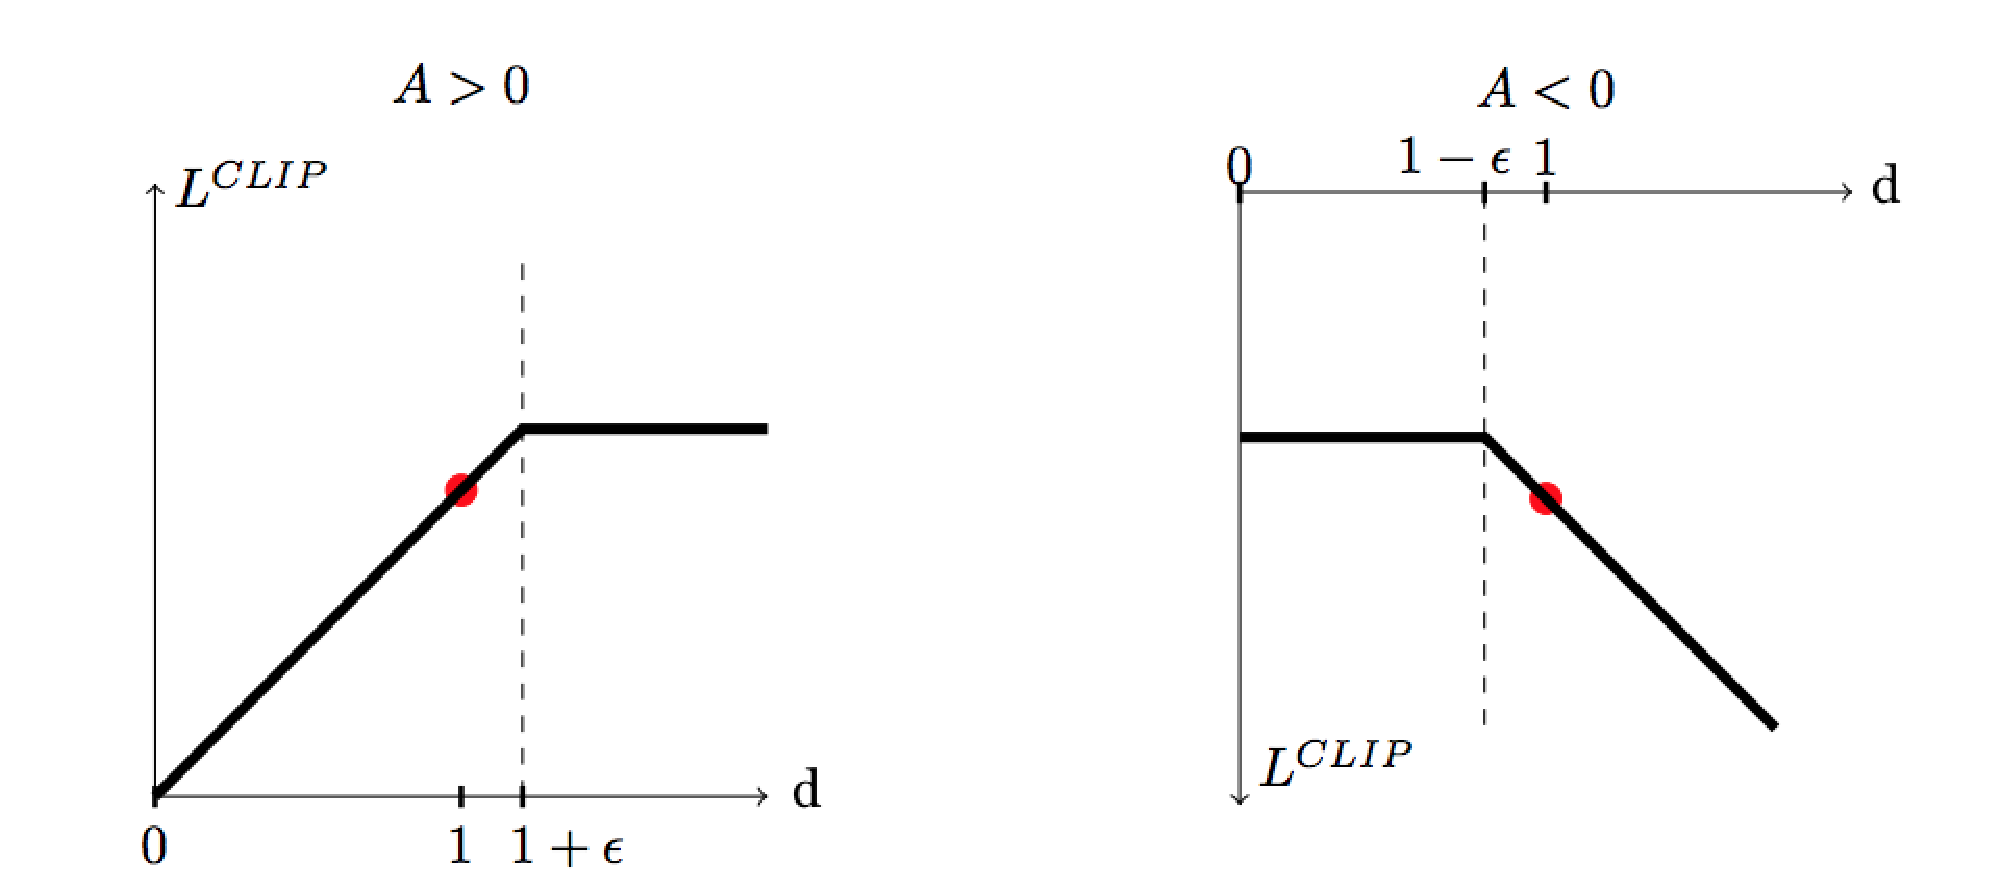
\includegraphics[width=0.8\textwidth]{./fig/ppo_clip}
  \captionsetup{width=1\textwidth}
  \caption{Comportamento da função $L^{CLIP}$ para valores de vantagem positivos (esquerda) e negativos (direita) \cite{ppo}, para atualizações em um único episódio.}
 \label{fig:ppoclip}
\end{figure}

Neste trabalho, a função de atualização do PPO é combinada com o termo de regularização baseado na entropia, definido na Seção \ref{sec:gae}. Além disso, um modelo parametrizado que estima a função de valor $V$ também é otimizado, caracterizando assim uma arquitetura Ator-Crítico \cite{suttonbarto}. A função de atualização toma então a forma da Equação \ref{eqn:totalloss}, onde $c$ é uma constante que regula a escala do termo de entropia e $L^{VF}$ é a função de custo do modelo da função de valor.

\begin{equation}
\label{eqn:totalloss}
L^{CLIP + VF + H}(\theta) = \mathop{{}\mathbb{E}}{}_t [L^{CLIP} - L^{VF} + cH(\pi(s_t; \theta))]
\end{equation}

Por fim, o algoritmo PPO com função de atualização limitada é apresentado no Algoritmo \ref{alg:ppoclip} \cite{achiam}, onde N é o tamanho do lote de treinamento do algoritmo de otimização.

\medskip
\begin{center}
\begin{minipage}{0.92\textwidth}
\begin{algorithm2e}[H]
 \DontPrintSemicolon
 \Entrada{parâmetros da política inicial $\theta_0$, limiar de corte $\epsilon$}
 \Para{$k= 0, 1, 2, ...$}
   {Colete um conjunto de trajetórias $D_k$ com política $\pi_k = \pi(\theta_{k})$ \\
    Estime a função de vantagem $A_{t}^{GAE(\gamma, \lambda)}$ \\
    Calcule a atualização da política \\
    \hspace{2cm}$\theta_{k+1} = arg \max_{\theta} L^{CLIP + VF + H}(\theta_k)$ \\
    executando N passos do gradiente ascendente, onde \\
    \hspace{2cm}$L^{CLIP + VF + H}(\theta_k) = \mathop{{}\mathbb{E}}{}_t [L^{CLIP} - L^{VF} + cH(\pi(s_t; \theta))]$ 
   }
\caption{PPO com função de atualização limitada \label{alg:ppoclip} }
\end{algorithm2e}
\end{minipage}
\end{center}



\section{Motivação Intrínseca}
\label{sec:curiosidade}

Um dos maiores desafios do aprendizado de reforço é aplicação de suas técnicas em ambientes reais. Dois principais problemas podem ser destacados: generalização e modelagem de recompensa. O primeiro diz respeito a capacidade de um agente treinado em uma configuração específica, ou um simulador, ser capaz de atuar de forma satisfatória em diferentes configurações, como em um manipulador robótico real. O segundo diz respeito à dificuldade de se modelar funções de recompensa que guiem um agente a agir de forma a completar uma determinada tarefa.

A sensibilidade dos algoritmos de aprendizado por reforço ao segundo problema faz com que, na maioria das vezes, o agente aprenda a explorar falhas do simulador ou falhas da modelagem da recompensa e simplesmente ignorar a tarefa que lhe foi dado. Além disso, a modelagem da função de recompensa para tarefas minimamente complexas é uma tarefa difícil \cite{dexterity, ng, deepLoco}. A alternativa natural é o uso de recompensas esparsas, recompensando o agente apenas no momento em que ele completou a tarefa desejada, por exemplo. Porém, em ambientes onde a recompensa é esparsa ou inexistente, aprender boas políticas por tentativa e erro é uma tarefa extremamente difícil. Nessas situações, não existe um direcionamento claro de como o agente deve modificar sua política a fim de maximizar sua recompensa. Além disso, técnicas de exploração clássicas comumente utilizam distribuições de probabilidade sobre as ações que não levam em consideração guiar o agente a estados inexplorados, o que pode não ser suficiente para a descoberta de políticas que são capazes de alcançar o objetivo determinado \cite{pathak}.

Como saída para este problema é possível encorajar o agente a explorar melhor o ambiente e aprender novas habilidades recompensando-o de forma intrínseca, ou seja, independente da recompensa fornecida pelo ambiente (extrínseca). Uma forma de modelar a motivação intrínseca é através da geração um sinal de recompensa proporcional ao nível de surpresa do agente em relação aos estados que ele observa \cite{curiosityoriginal, pathak}. Para isso, um modelo de futuro é responsável por prever o próximo estado $s_{t+1}$ dados o estado atual $s_t$ e a ação $a$ executada, como mostra a Equação \ref{eqn:forward}.

\begin{equation}
\label{eqn:forward}
\hat{s}_{t+1} = f(s_t, a_t; \theta_F)
\end{equation}

Dado o real estado futuro $s_{t+1}$ é calculado o erro de predição, ou seja, a função de custo do modelo, como mostra a Equação \ref{eqn:curiosityloss}.

\begin{equation}
\label{eqn:curiosityloss}
L_F(s_{t+1}, \hat{s}_{t+1}) = \frac{1}{2}\|\hat{s}_{t+1} - s_{t+1}\|_2^2
\end{equation}

O erro de predição é então multiplicado por uma constante $\eta$ que ajusta sua escala. Por fim, o valor é adicionado à recompensa do ambiente ($r^e$) como recompensa intrínseca, como mostra a Equação \ref{eqn:curiosityreward}.

\begin{equation}
\label{eqn:curiosityreward}
r_t = r^e_t(s_t, a, s_{t+1}) + \eta L_F
\end{equation}